\documentclass[main.tex]{subfiles}

\begin{document}

\subsection{Secondo esercizio}

\begin{figure}[H]
\centering
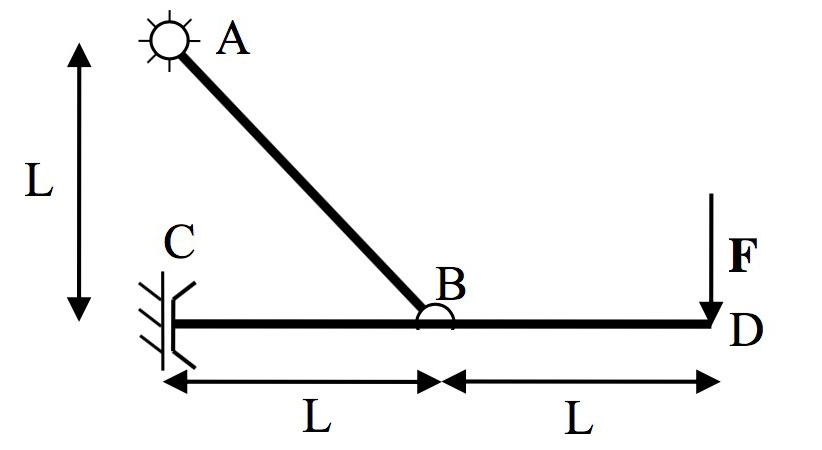
\includegraphics[width=0.75\textwidth]{2014-2207-2.jpg}
\end{figure}

La struttura in figura è soggetta al solo carico verticale $F$.

Si chiede di calcolare:

\begin{enumerate}
\item Le reazioni vincolari in C.
\item Le azioni interne nell’asta CD.
\end{enumerate}

\clearpage

\subsection{Soluzione secondo esercizio (non verificata)}

\subsubsection{Osservazioni}

\begin{enumerate}
\item La struttura è composta da un'asta e 2 vincoli: un pattino ed un pendolo (o biella).
\end{enumerate}

\subsubsection{Analisi preliminare di isostaticità}
Verifico che $gdl_{tot} = gdv_{tot}$:
\begin{figure}[H]
  \begin{subfigure}[b]{.5\textwidth}
  \centering
  \[
  	gdv: \begin{cases}
		gdv_{pattino} = 2\\
		gdv_{biella} = 1
  	\end{cases}
  \]
  \caption{Gradi di vincolo del sistema.}
  \end{subfigure}
  \hfill
  \begin{subfigure}[b]{.5\textwidth}
  \centering
  \[
  	gdl: \begin{cases}
  		gdl_{asta} = 3\\
  	\end{cases}
  \]
  \caption{Gradi di libertà del sistema.}
  \end{subfigure}
  \caption{Verifica preliminare di isostaticità.}
\end{figure}

\subsubsection{Primo punto}

\paragraph{Analisi dei vincoli esterni}

\begin{figure}[H]
\centering
\resizebox{.5\textwidth}{!}{% First image 2015 06 29

\begin{tikzpicture}

  \tiny


  \point{c}{0}{0}
  \point{c1}{0}{0.8}
  \point{c2}{-0.8}{0}
  \point{a}{2-1.41421}{1.41421}
  \point{a1}{2-1.41421}{0.8+1.41421}
  \point{d}{2}{0}
  \point{b}{2+1.41421}{-1.41421}
  \point{b1}{2+1.41421}{-1.41421-1.3}

  \beam{2}{c}{d}[0][1];
  \beam{2}{a}{b};

  \load{1}{a}[180][0.5]
  \load{1}{a1}[270][0.5]

  \load{2}{c}
  \load{1}{c}[180][0.5]
  \load{1}{c}[270][0.5]

  \load{1}{b1}[90][1]

  \notation{1}{c}{$\vec{M}_C$}[below right]
  \notation{1}{c}{$\vec{H}_C$}[below left]
  \notation{1}{c}{$\vec{V}_C$}[above right]

  \notation{1}{a}{$\vec{H}_A$}[below left]
  \notation{1}{a}{$\vec{V}_A$}[above right]

  \notation{1}{b}{$\vec{F}$}[below right]

  % \notation{1}{a1}{$\vec{H}_A$}
  % % \notation{1}{d1}{$\vec{R}_D$}
  % % \notation{1}{b1}{$\vec{H}_B$}[below left]
  % \notation{1}{c1}{$\vec{F}$}[above left]

  %  % \support{3}{o};

  %  % %Degrees
  %  % \notation{1}{o}{$\alpha$}[above];
  %  % \notation{1}{a}{$\beta$}[above];

  %  % \notation{5}{o}{a}[$a$];
  %  % \notation{5}{a}{b}[$b$];
  %  % \notation{5}{o}{b}[$c$];

\end{tikzpicture}}
\caption{Analisi dei vincoli esterni}
\end{figure}

\[
\begin{cases}
	H_A = - H_C\\
	V_A = F\\
	M_C + LH_A + 2LF = 0
\end{cases}
\]

\paragraph{Considerazioni sulla reazione assiale della biella}
La biella trasmette unicamente la reazione assiale, che è inclinata di $45\deg$ dato che i due lati sono entrambi lunghi $L$. Le componenti cartesiane di questa reazione assiale sono quindi uguali: $R_{C_x} = R_{C_y}$.

\begin{figure}[H]
\centering
\resizebox{.5\textwidth}{!}{% First image 2015 06 29

\begin{tikzpicture}

  \tiny

  \point{a}{0}{0}
  \point{c}{1}{0}
  \point{b}{2}{2}
  \point{d}{1}{1}

  \beam{2}{a}{b}

  \load{1}{b}[180][0.5]
  \load{1}{a}[180][0.5]
  \load{1}{a}[90][1]

  \load{1}{d}[0][1]
  \load{1}{d}[-90][1]

  \notation{1}{a}{$\vec{F}$}[below left]
  \notation{1}{a}{$2\vec{F}$}[above left]

  \notation{1}{b}{$\vec{F}$}[above left]

  \notation{1}{d}{$\vec{R}_{D_x}$}[below right]
  \notation{1}{d}{$\vec{R}_{D_y}$}[below left]

\end{tikzpicture}}
\caption{Sforzo normale nell'asta AB.}
\end{figure}

\[
\begin{cases}
	R_{C_x} = R_{C_y}\\
	R_{C_x} = H_A\\
	R_{C_y} = -V_A\\
	V_A = -H_A = F\\
\end{cases}
\]

Sostituisco queste relazioni nel sistema precedente e risolvo l'equazione del momento in A:

\[
	M_C - LF + 2LF = 0
	\Longrightarrow
	M_C = -LF
\]

\begin{figure}[H]
\centering
  \[
  	C: \begin{cases}
		H_C = F\\
		M_C = -LF
  	\end{cases}
  \]
  \caption{Reazioni vincolari in C.}
\end{figure}

\subsubsection{Secondo punto}
Essendo l'asta posizionata orizzontalmente, l'asse normale e  tangente corrispondono rispettivamente con ascisse ed ordinate.

\[
	C: \begin{cases}
		N = F\\
		T = 0\\
	\end{cases}
	\qquad
	B: \begin{cases}
		N = F\\
		T = F\\
	\end{cases}
	\qquad
	F: \begin{cases}
		T = F\\
	\end{cases}
\]

\paragraph{Sforzo normale baricentrico} Nel tronco di asta CB lo sforzo normale risulta negativo, poiché di \textbf{contrazione}. Nel tronco di asta BD invece non avviene sforzo normale.

\begin{figure}[H]
\centering
\resizebox{.5\textwidth}{!}{% First image 2015 06 29

\begin{tikzpicture}

  \tiny


  \point{c}{0}{0}
  \point{a}{0}{1}
  \point{b}{1}{0}
  \point{d}{2}{0}

   \beam{2}{c}{d}[0][1];

  \internalforces{c}{b}{1}{1}[0][blue];

\end{tikzpicture}}
\caption{Sforzo normale nell'asta CD.}
\end{figure}

\paragraph{Taglio} Nel tronco di asta CB non avviene taglio. Nel tronco BD invece, le forze $T_A$ ed $F$ impongono una rotazione \textbf{oraria}, e quindi è positiva.

\begin{figure}[H]
\centering
\resizebox{.5\textwidth}{!}{% First image 2015 06 29

\begin{tikzpicture}

  \tiny


  \point{c}{0}{0}
  \point{c1}{0}{0.8}
  \point{c2}{-0.8}{0}
  \point{a}{2-1.41421}{1.41421}
  \point{a1}{2-1.41421}{0.8+1.41421}
  \point{d}{2}{0}
  \point{d1}{2-0.8}{0}
  \point{b}{2+1.41421}{-1.41421}
  \point{b1}{2+1.41421}{-1.41421-1.3}

  \beam{2}{a}{b};

  \internalforces{a}{d}{-0.707}{-0.707}[0][blue];
  \internalforces{d}{b}{0.707}{0.707}[0][red];

\end{tikzpicture}}
\caption{Taglio nell'asta CD.}
\end{figure}

\paragraph{Momento flettente} Partendo da D, che impone un taglio $F$ dall'alto verso il basso, possiamo vedere che le fibre tese risultano sul lato superiore dell'asta. Il momento imposto da $F$ raggiunge il massimo nel punto B $M_{max} = LF$, in cui viene applicata una forza $F$ indirizzata in senso opposto che porta il momento a raggiungere lo zero linearmente in E.
\\
\\
Percorrendo il percorso a ritroso, partendo da E, è possibile ottenere lo stesso risultato.

\begin{figure}[H]
\centering
\resizebox{.5\textwidth}{!}{% First image 2015 06 29

\begin{tikzpicture}

  \tiny


  \point{c}{0}{0}
  \point{c1}{0}{0.8}
  \point{c2}{-0.8}{0}
  \point{a}{2-1.41421}{1.41421}
  \point{a1}{2-1.41421}{0.8+1.41421}
  \point{d}{2}{0}
  \point{d1}{2-0.8}{0}
  \point{b}{2+1.41421}{-1.41421}
  \point{b1}{2+1.41421}{-1.41421-1.3}

  \beam{2}{a}{b};

  \internalforces{a}{d}{0}{-0.707}[0][red];
  \internalforces{d}{b}{-0.707}{0}[0][red];

\end{tikzpicture}}
\caption{Momento flettente nell'asta CD.}
\end{figure}

\end{document}